\documentclass{beamer}

\title{Summer project presentation}
\subtitle{Or why we got paid}
\author{M.Kawalec, \\ D.Mallows}
\date{\today}
\usetheme{Warsaw}

\begin{document}
  \frame{\titlepage}

  \begin{frame}
    \frametitle{Table of Contents}
    \tableofcontents
  \end{frame}

  \begin{frame}
    \section{T analysis}
    \frametitle{T production}
    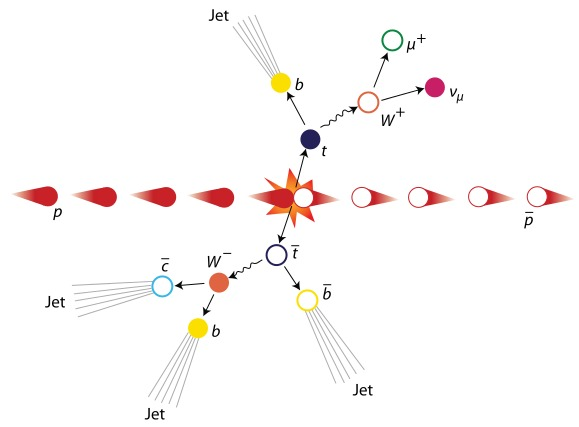
\includegraphics[height=0.89\textheight]{ttbar.jpg}
  \end{frame}
  \begin{frame}
    \section{YODA}
    \frametitle{YODA's main capabilities} 
      \begin{itemize}
        \item Fully on-line bin management \pause
        \item Transparent bin management \pause
        \item Good scaling \pause
        \item Easliy extendable with different classes
      \end{itemize}
  \end{frame}
  \begin{frame}
      \frametitle{fill() operations}
      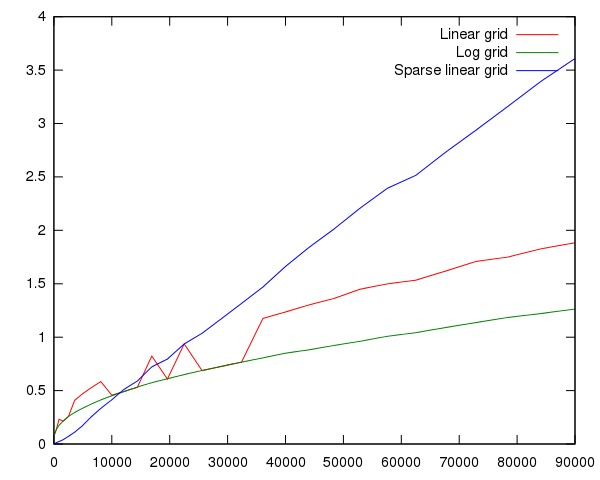
\includegraphics[height=0.89\textheight]{1.jpg}
  \end{frame}
  \begin{frame}
    \frametitle{add/rem operations}
    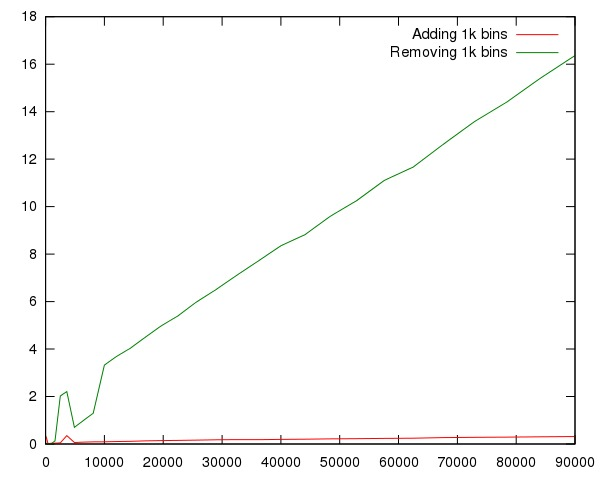
\includegraphics[height=0.89\textheight]{2.jpg}
  \end{frame}
  \begin{frame}
    \frametitle{rebin() all bins}
    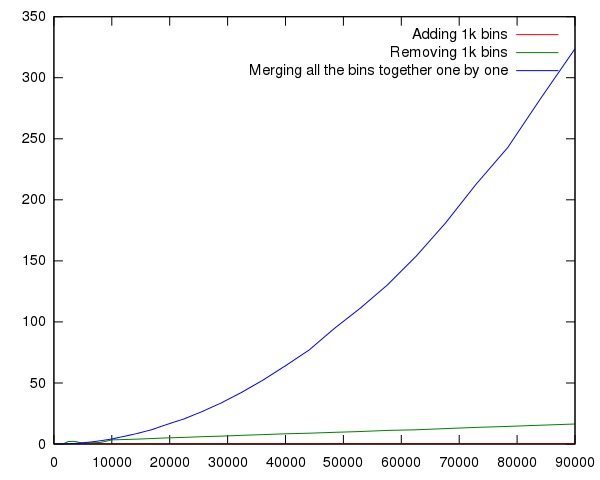
\includegraphics[height=0.89\textheight]{2a.jpg}
  \end{frame}
\end{document}
